\chapter{Related Work and Background}\label{ch2:related-work-background}

In this thesis, we have not created novel models or datasets but have rather curated preexisting datasets and retrained a state-of-the-art CNN. Data curation has been an essential part of our work as the datasets' YouTube videos are subject to modifications over time. These modifications are in terms of the videos being taken down from YouTube or the required 1280$\times$720 pixel (720p) resolution versions of them becoming unavailable, etc. The curation process included action items like downloading and training only on 720p versions of the datasets' videos so as to minimize the chances of running into training errors, etc., as explained in section~\ref{sec2:data}. As for simulating the 3D video chat experience itself, we linked-up the API of OpenFace 2.2 --- a preexisting head pose estimation model --- to the MPI inference procedure so the MPI inference may generate novel views rendered in the head pose evaluated by OpenFace 2.2, as explained in section~\ref{sec3:implementation}

This chapter explores related work in two areas: MPIs and 3D video chat, while providing clarifications on background concepts along the way. The research papers of particular interest to us as far as the MPI component of our work is concerned are 2018's Zhou et al.~\cite{zhou2018stereo} and 2020's Tucker and Snavely~\cite{single_view_mpi}, which we consider to be our base papers. This is because we have attempted to adapt and apply Tucker and Snavely's work to the purposes of video chatting and their work directly draws from Zhou et al. We have also sought to differentiate 2016's Flynn et al.~\cite{deep_stereo_2016} and Kalantari et al.~\cite{kalantari_2016} from Zhou et al. as it, in turn, is heavily inspired by them and surpasses them performance-wise. As for progress in the field of 3D video chat, we have mentioned the yet to be released state-of-the-art 3D video chat system: Google's Project Starline, among other projects.

\section{Learning MPIs}\label{sec:approach} 

Some of the major challenges of high-quality novel view synthesis include synthesizing pixels occluded in one or more of the provided views, disentangling and localizing pixels at/near the boundaries of foreground and background objects, localizing pixels at transparent, translucent, or reflective surfaces, etc. Moreover, whereas interpolating novel views at desired viewpoints lying in between the given views is easier to achieve compared to extrapolating significantly beyond the baselines (distances between camera centers) of input viewpoints, these challenges are going to be present in either case. So far, it has been found that learning view synthesis is the way to go for tackling all these challenges in one shot. Before the Machine Learning (ML) boom in Computer Vision (CV) circles in 2012, convolutional filters had to be handcrafted and carefully layered one on top of the other before input views could be subjected to them and various types of features could be extracted to render novel views. All the aforementioned view synthesis challenges had to be manually targeted by way of devising various combinations of filters for each complication. This meant a high proportion of artifacts induced in novel views would be left unresolved. Since 2012, prominently and to the delight of the CV community, the need to handcraft filters was obviated by ML models that learned to design all required convolutional filters on their own in their various layers. These self-learnt filters are defined by the constantly improving weights and biases in each neuron of the network layers and are mostly specific to the datasets they are trained on, with some degree of generalizability to other datasets. If trained well under effective hyperparamter tuning, learnt filters can evolve to surpass manual filters in redressing occlusion, transparency, reflection, and other image synthesis problems.

View synthesis lends itself to being a semi-well-posed to well-posed learning problem where two or more images of a scene can be shot and an ML model can be exposed to one of more of these images while being expected to predict one or more of the remaining views that have been withheld from it. The quantitative difference between the corresponding predicted and withheld (ground truth) views will then be the loss that the ML training seeks to minimize. Since, end-to-end view synthesis without an intermediate representation is still largely unrealized, the popular way to synthesize novel views is to learn an intermediate representation of the scene common to the input views and use this intermediate representation to render novel views. The MPI intermediate representation has proven to be one the most effective representations for this purpose with implications as significant as real-time high-quality view synthesis. The roots of the MPI representation may be traced back to seminal work such as 1996's \cite{collins_space-sweep_1996} 1998's \cite{fft} and 1999's \cite{fft} --- the 1996, 1998, and 1999 papers. The 1996 paper first perfected the concept of plane sweep volumes, the 1998 paper introcuded layered depth images and the 1999 paper the actual MPI representation itself.
come back to come bcak and drive up thse gat eto come back and take down and take irt back up to the coming month and taeke it up bring it back to get it doen to coming permanent solutij andf come back and benglwts xoemhvfanadI thij I know hwo to ome abck anmd so they come down to the bring  and bring back dow to this situastio sand come back up to this case and down to this awesome ness and ope fuk ytsoend this timwe and lau dow to coming back to thisd lllcolbalt colamp did nothid but bundle adjustment sndf alignke and I wouf like to tske a lok at tho and 

Kalantari interpolates (fills in) novel views in the 8x8 (u,v) view grid of a lytro camera this grid is that of microlens arrays that has microlensing arrays 
The model the 

MPI scene representation is similar to Layered Depth Image (LDI) scene representation introduced by \cite{layered_depth_images}. Both MPI and LDI consist of a series of fronto-parallel planes facing the reference camera of one of the given images and placed at different depths from it. These planes contain the RGB information of the original pixels of the image(s), segregated according to depth. The difference between LDI and MPI is that MPI has alpha masking effects at each layer as it is generated with alpha transparency maps for each layer. Also, MPI has fixed depths for each layer as opposed to the varying layer depths of LDI.

MPI scene representation is similar to Layered Depth Image (LDI) scene representation introduced by \cite{layered_depth_images}. Both MPI and LDI consist of a series of fronto-parallel planes facing the reference camera of one of the given images and placed at different depths from it. These planes contain the RGB information of the original pixels of the image(s), segregated according to depth. The difference between LDI and MPI is that MPI has alpha masking effects at each layer as it is generated with alpha transparency maps for each layer. Also, MPI has fixed depths for each layer as opposed to the varying layer depths of LDI. 

\begin{figure}[!h]
    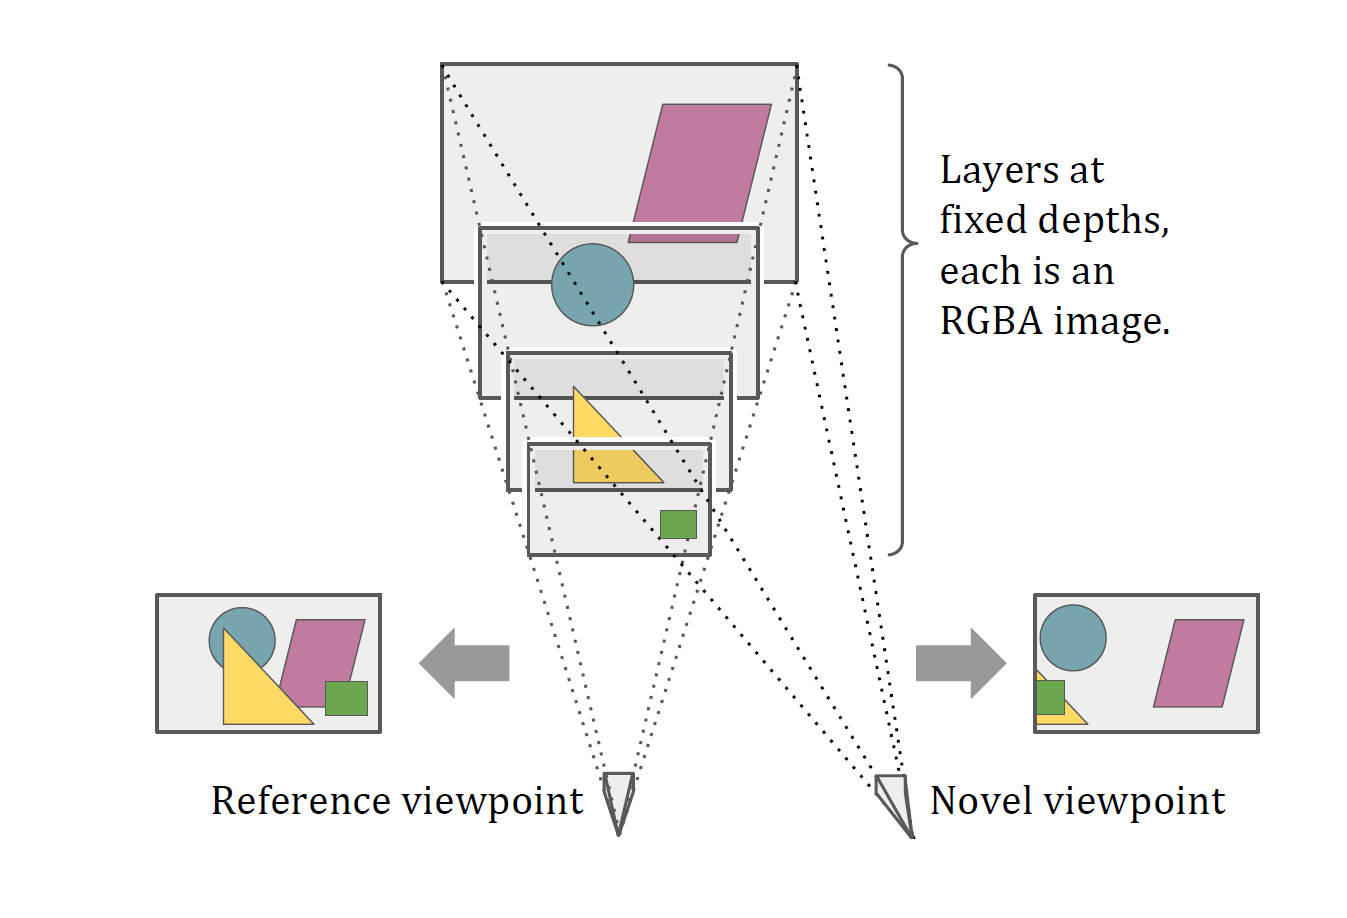
\includegraphics[width=1\columnwidth]{figures/mpi-layered-representation.png}
    \caption{Fronto-parallel planes in MPI layered representation}
    \label{fig:mpi-layered-representation}
\end{figure}
Fig 3. Example of fronto-parallel planes

The 2018's Stereo MPI and 2020's Single-View MPI papers have the similar training procedures of suppressing some frames from a video clip as ground truth, attempting to predict these frames and finally minimizing various loss metrics between the rendered frame and the suppressed frame.

\subsection{The 1999 paper}\label{subsec2:1999}
\subsubsection{The 1999 paper}\label{subsubsec2:1999}

The 1999 MPI paper first introduced the MPI representation for purposes of stereo matching, otherwise called disparity mapping. In this paper the authors used MPIs for matte separation of foreground and background in which they sample the 3D Cartesian space into a disparity space where a 3D point [x y z] would map to [x y 1 d]. Since disparity maps are a byproduct of the 2020 MPI model, it behoves us to explain here what they are. Disparity is nothing by the pixel distance between any two corresponding/matching pixels in stereo image pair. This correspondence or finding if the pixel occurs in both images of the stereo pair the can be determined by first running feature detection algorithms like SIFT and then subjugating the extracted features to realignment and finally to these depth prediction algorithms.

Stereo Matching is one of the core technologies in computer vision, which recovers 3D structures of real world from 2D images. It has been widely used in areas such as autonomous driving, augmented reality and robotics navigation. Given a pair of rectified stereo images, the goal of Stereo Matching is to compute the disparity for each pixel in the reference image, where disparity is defined as the horizontal displacement between a pair of corresponding pixels in the left and right images.
    
\begin{figure}[!h]
    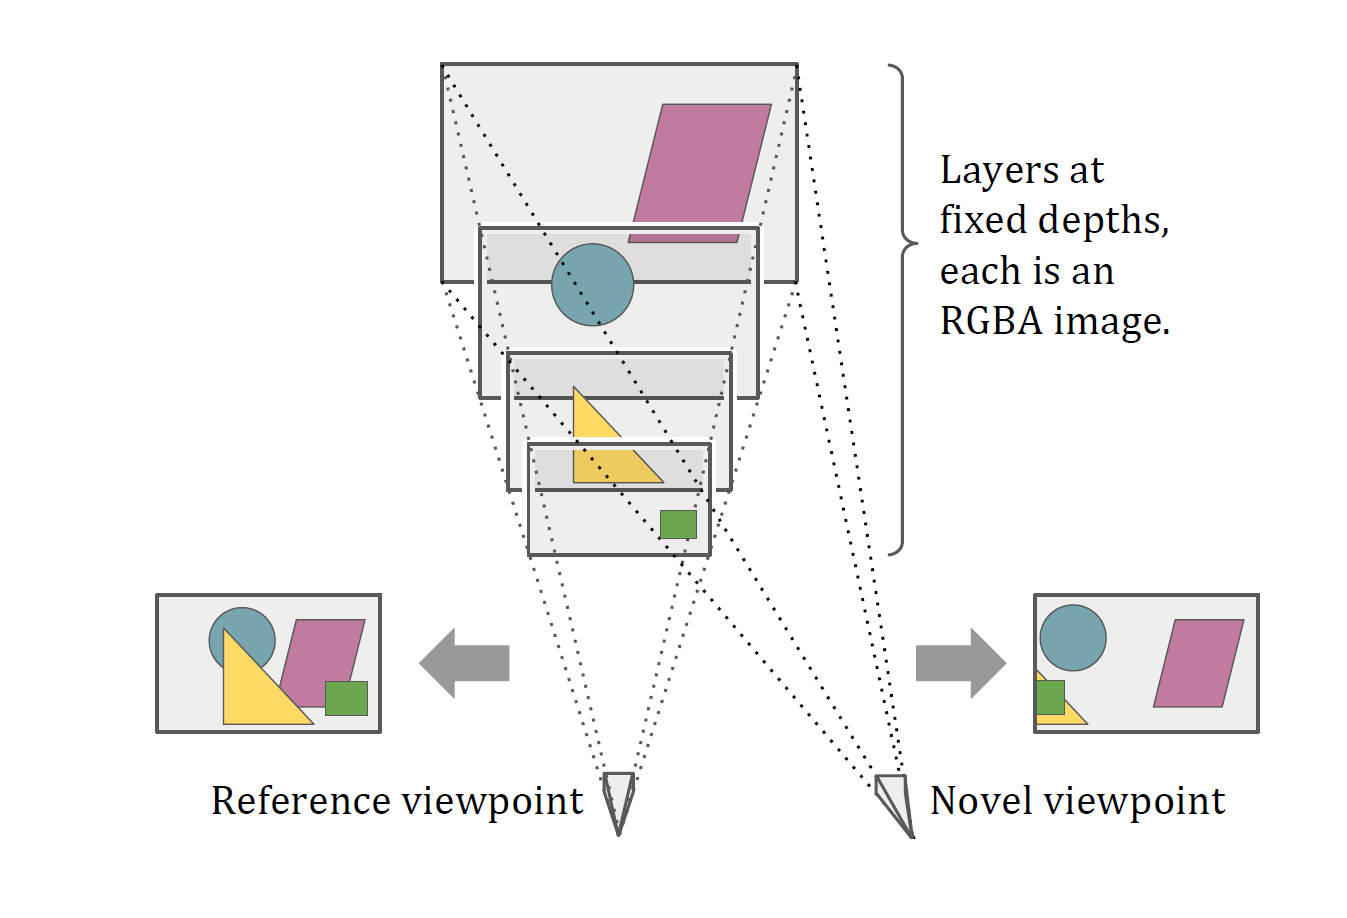
\includegraphics[width=1\columnwidth]{figures/mpi-layered-representation.png}
    \caption{Fronto-parallel planes in MPI layered representation}
    \label{fig:mpi-layered-representation}
\end{figure}
Fig 3. Example of fronto-parallel planes

To examine the novel stereo correspondence algorithm's features, the authors conducted a modest set of experiments on certain synthetic stereo datasets, evaluating both the algorithm's basic behavior and its performance on mixed pixels. Visualizing opacities/transparencies is critical for comprehending and validating the algorithm. As a result, the writers selected color stimuli. The authors began by creating a typical random-dot stereogram with k = 5 pictures, in which the camera geometry and filled disparity planes result in integral pixel shifts. This sample contains no pixels that are partially translucent. The first eight columns indicate the estimated colors and opacities of the eight disparity planes in (x, y, d) space.

While preliminary experimental results are intriguing, recovering correct depth, color, and opacity estimations simultaneously remains a difficult task. On the other hand, is to recover a poorly populated color and opacity volume. This has the advantage of accurately modeling mixed pixels and occlusion effects, allowing them to integrate photos taken from extremely dissimilar angles of view. It significantly complicates the estimation problem, as the number of free parameters frequently exceeds the number of data, necessitating the use of smoothness constraints and other previous models. To address these issues, it may be necessary to improve imaging and sensor models, or to work on a higher resolution picture grid.

The authors have created a novel framework for recovering disparities, hues, and opacities from several images concurrently. This framework enables them to cope with a variety of stereo matching issues that arise frequently, such as partially occluded regions and pixels that contain foreground and background color combinations. It promises to give higher-quality color and opacity estimations that can be used to extract foreground objects and blend real and synthetic imagery. This format can enable a far broader range of synthetic views than a single texture-mapped depth picture can in view interpolation applications.

 \subsection{The 2016 paper}\label{subsec2:2016}

Estimating 3D shape from multiple posed images is a fundamental task in computer vision and graphics, both as an aid to image understanding and as a way to generate 3D representations of scenes that can be rendered and edited. The authors aim to solve the related problem of new view synthesis, a form of image-based rendering (IBR) where the goal is to synthesize a new view of a scene by warping and combining images from nearby posed images. This can be used for applications such as cinematography, virtual reality, teleconferencing [4], image stabilization [19], or 3-dimensionalizing monocular film footage. Good approaches to IBR typically require the use of strong priors to fill in pixels where the geometry is uncertain, or when the target color is unknown due to occlusions The authors aim to solve the related problem of new view synthesis, a form of image-based rendering (IBR) where the goal is to synthesize a new view of a scene by warping and combining images from nearby posed images.
The authors' goal is to learn a model for predicting new viewpoints by directly minimizing the prediction error on the training set

To evaluate the model on view interpolation, the authors generated a novel image from the same viewpoint as a known image captured by the Street View camera.
The imagery from this prior work is quite different from the training images, as these prior images were taken with a handheld DSLR camera. Despite the fact that the model was not trained directly for this task, it did a reasonable job at reproducing the input imagery and at interpolating between them. These images were rendered in small patches, as rendering an entire image would be prohibitively expensive in RAM. The authors' current implementation does not fully exploit the convolutional nature of the model, so these times could likely be reduced to minutes or even seconds by a GPU implementation in the spirit of Krizhevsky, et al [20]

\begin{figure}[!h]
    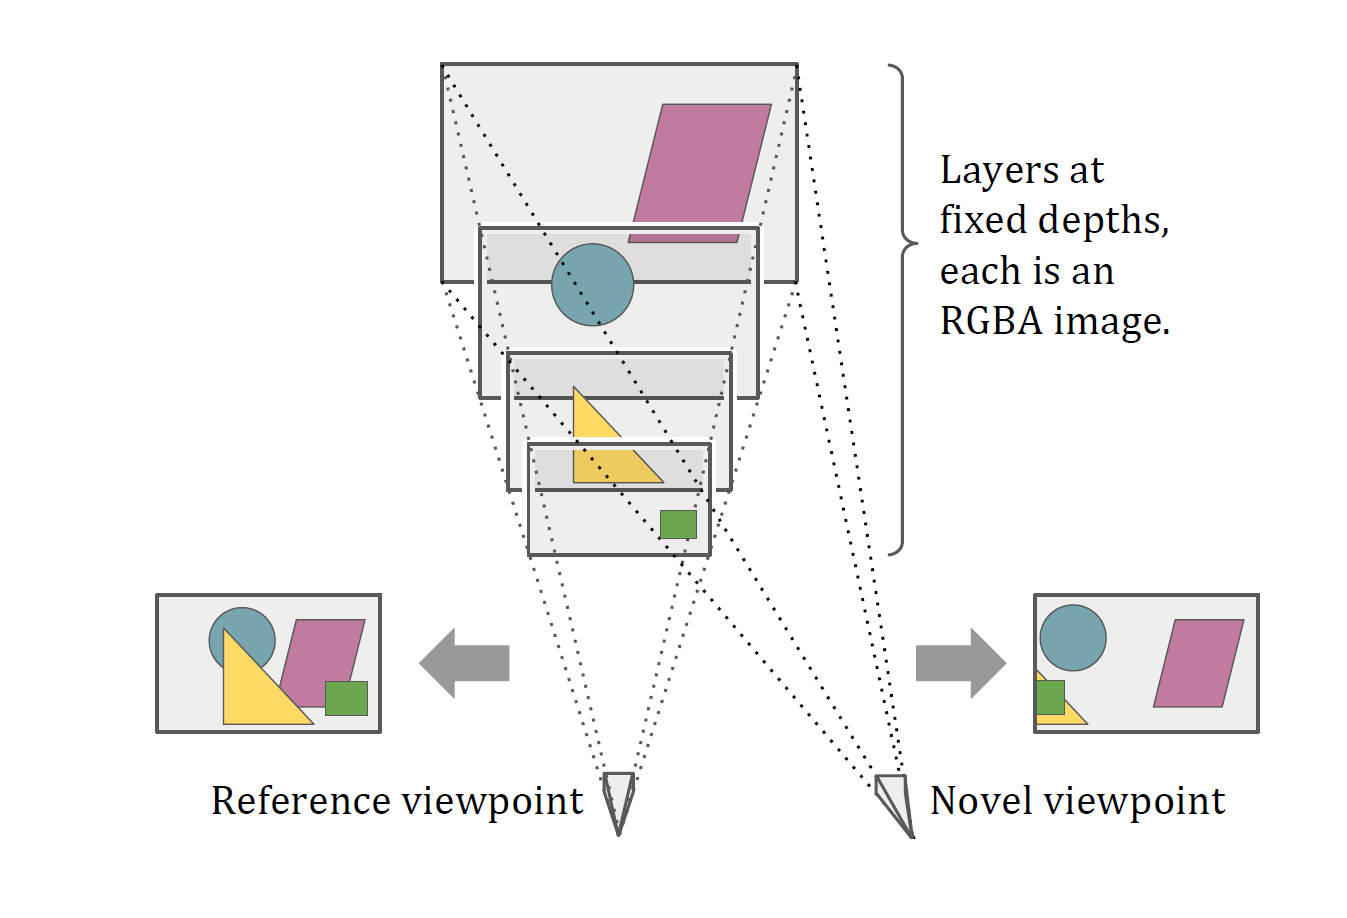
\includegraphics[width=1\columnwidth]{figures/mpi-layered-representation.png}
    \caption{Fronto-parallel planes in MPI layered representation}
    \label{fig:mpi-layered-representation}
\end{figure}
Fig 3. Example of fronto-parallel planes

The authors have shown that it is possible to train a deep network end-to-end to perform novel view synthesis. The authors' method currently requires reprojecting each input image to a set of depth planes; the authors currently use 96 depth planes, which limits the resolution of the output images that the authors can produce. Increasing the resolution would require a larger number of depth planes, which would mean that the network takes longer to train, uses more RAM and takes longer to run. This is a drawback shared with other volumetric stereo methods; the method requires reprojected images per rendered frame, rather than just once when creating the scene. The authors plan to explore pre-computing parts of the network and warping to new views before running the final layers

 \subsection{The 2018 paper}\label{subsec2:2018}

Motivated by the development of stereo cameras, this article investigates the difficulty of creating novel perspectives from such narrow-baseline image pairings. While most past work has focused on interpolating between a set of supplied views [Chen and Williams 1993], the authors concentrate on the problem of significantly extrapolating views beyond the two input images. This type of view extrapolation has a variety of uses in photography. The authors may seek to extend an IPD-separated stereo pair acquired with a VR180 camera to an entire set of views along a line, say half a meter in length, in order to achieve full parallax with a minimal range of head motion. The authors refer to this technique as stereo magnification, which involves extrapolating a view from a pair of input views. The authors require the ability to render pixels that are obscured and invisible in one of the input views. To overcome these issues, we will train our system to conduct view extrapolation from vast volumes of visual data, similar to recent work on view interpolation using deep learning [Flynn et al 2016; Kalantari et al 2016]. The authors seek a scene representation that can be predicted once given a pair of input views and then reused to predict a large number of output views, in contrast to past work that required prediction of each output view independently. The authors demonstrate that the learnt model generalizes to additional datasets without requiring retraining and is successful at amplifying the limited baseline of stereo vision acquired by cell phones and stereo cameras. Multiplane Images are a novel type of scene representation that can be used to do vision synthesis. A novel use of online video to the study of view synthesis, namely view extrapolation

\begin{figure}[!h]
    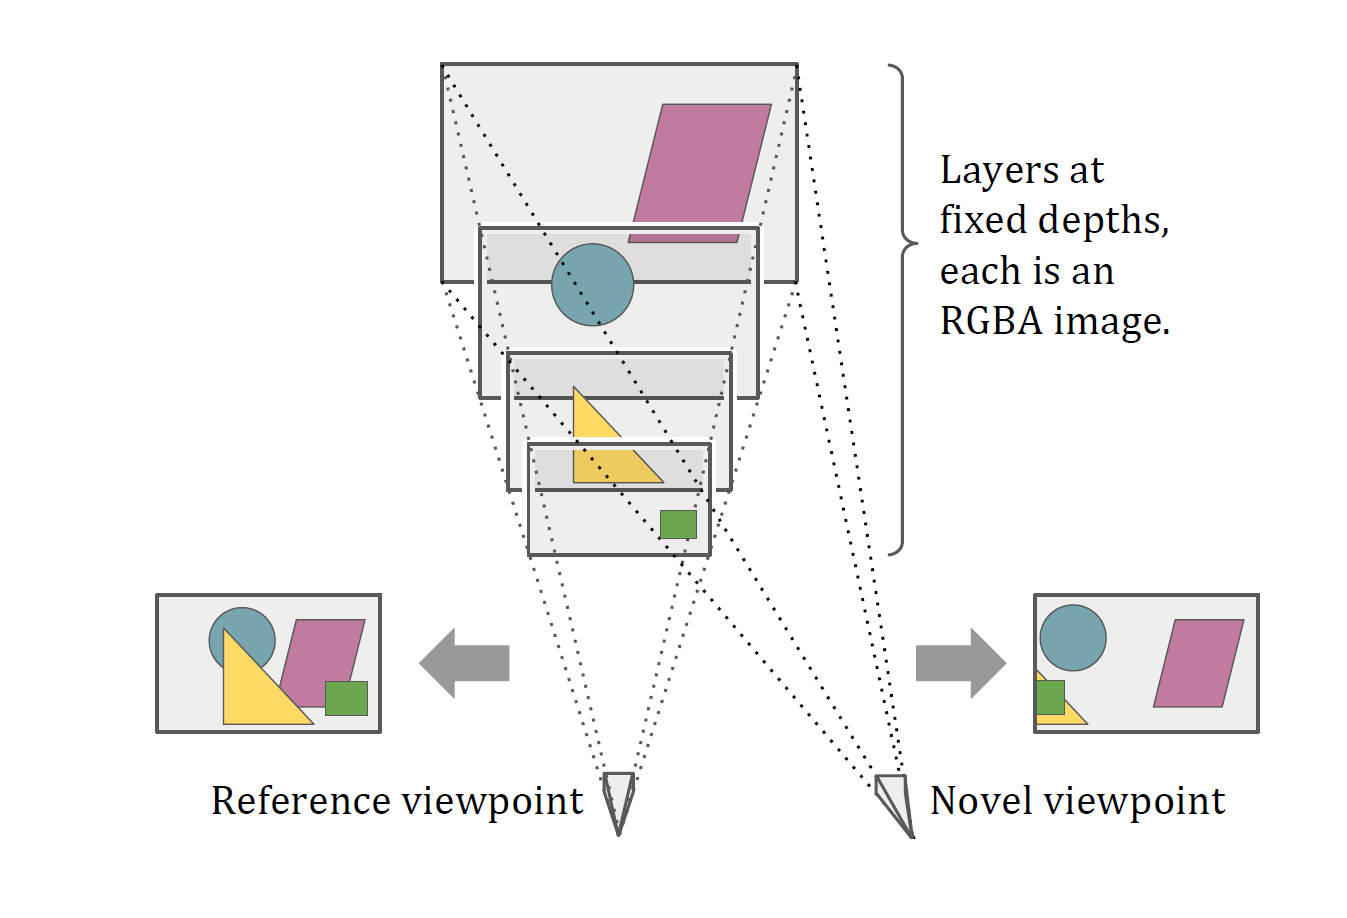
\includegraphics[width=1\columnwidth]{figures/mpi-layered-representation.png}
    \caption{Fronto-parallel planes in MPI layered representation}
    \label{fig:mpi-layered-representation}
\end{figure}
Fig 3. Example of fronto-parallel planes

An MPI is similar to the Layered Depth Image (LDI) representation proposed by Shade et al. [Shade et al 1998], except that the pixels in each layer are fixed at a specific depth, and the authors encode visibility using an alpha channel per layer. The authors' depiction is reminiscent of the multiplane camera pioneered at Walt Disney Studios and widely utilized in traditional animation. [2017, Wikipedia] A scene is made of a sequence of partially transparent layers at varying distances from the camera in both systems. Along with the input photos I1 and I2, the authors include their associated camera parameters. The predicted scene's reference coordinate frame is centered on the camera in the first input picture I1 (i.e., p1 is fixed to be the identity pose). The authors compute a plane sweep volume (PSV) that reprojects I2 into the reference camera at a set of D fixed depth planes in order to encode the pose information from the second input picture I2. The authors chose these depth planes to correspond to the output MPI's depth planes. The output of this plane sweep computation is a stack of reprojected pictures I1,. The network output might simply be a single RGBA image for each depth plane, with the color image capturing the scene's look and the alpha map encoding visibility and transparency. The authors assume that the scene's color information can be accurately modeled using only two images: a foreground and a background image, where the foreground image is the reference source I1 and the background image is predicted by the network and is intended to capture the appearance of hidden surfaces.

The network generates the following values: 1) an alpha map d for each plane, 2) a global RGB background image Ib, and 3) a blending weight image wd for each plane indicating the foreground and background layers' relative proportions at each pixel. If the authors forecast D depth layers with each layer having a resolution of W H, then the total number of output parameters is W H (2D + 3).
These values can be converted to an MPI value. The authors can generate a novel view using the MPI representation in relation to a reference frame. It accomplishes this by performing a planar transformation on the RGBA image for each plane, followed by an alpha-composition of the changed images into a single image in reverse order. Both the planar transformation and alpha composition are distinct operations that can be integrated into the remainder of the learning pipeline. The authors retrieve each pixel in the target MPI plane using typical inverse homography [Hartley and Zisserman 2003]. The authors can retrieve the color and alpha values for each target pixel [ut, vt ] by locating its correspondence in the source image [us, vs ]. The authors derive the expected target view by alpha compositing the color images in back-to-front order using the standard over operation after applying the planar transformation to each MPI plane [Porter and Duff 1984].

The authors can train a network to predict MPIs matching the view synthesis target given the MPI inference and rendering process. Although the pictures and MPI have a spatial resolution of 1024 576, the model may be fully convolutional applied to any resolution at test time. While many videos on YouTube are unsuitable for the purposes, the writers discovered a surprising amount of relevant content across a variety of video categories. Real estate footage is one such category. The typical real estate video consists of a succession of views of inside and exterior locations. The authors chose to create a dataset using real estate videos in order to obtain a big and diversified set of multi-view training images. The remainder of this section discusses the authors' dataset, which includes over 7,000 video clips ranging in duration from one to ten seconds, as well as the camera position, orientation, and field of vision for each frame in the sequence. To create this dataset, the authors created a pipeline for mining appropriate YouTube video. The authors developed a pipeline for extracting appropriate YouTube video. This pipeline is divided into four distinct stages: 1) selecting a set of candidate videos to download, 2) running a camera tracker on each video to estimate an initial camera pose for each frame and subdivide the video into distinct shots/clips, 3) performing a full bundle adjustment to derive high-quality poses for each clip, and 4) filtering to remove any remaining unsuitable clips.

After training on a vast and diverse dataset, the multiplane image-based view synthesis system is capable of handling both interior and outdoor scenarios.
This may indicate that depth judgments are being made at an insufficiently local level. The authors described a novel format, training setup, and approach for extracting views from video data. The authors believe that this framework can be applied to a range of different tasks, including extrapolating from several input images or from a single one, and producing lightfields that enable view movement in multiple dimensions.

 \subsection{The 2020 paper}\label{subsec2:2020}

Taking a photograph and being able to move the camera around is an enticing way to bring a scene to life. It requires an understanding of the scene's three-dimensional structure, reasoning about occlusions and what might be behind them, and rendering high-quality, spatially consistent new views in real time. The authors use the multiplane image (MPI) representation, which is capable of modeling disocclusions and non-Lambertian effects, generates spatially consistent views, is well-suited for creation via convolutional networks, and can be rendered efficiently in real time [37]. A special issue occurs when overseeing such a system via view synthesis, due to the uncertainty in the input data's global scale. The authors address this issue with a method of scale invariant view synthesis that makes use of sparse point sets generated during the training data generation process. The authors present an edge-aware smoothness loss that prevents depth maps created from predicted MPIs from becoming excessively fuzzy, even in the absence of depth supervision.

While the authors' purpose is view synthesis rather than depth prediction, they can easily generate disparity maps from the MPIs and use these to assess depth performance. The authors conduct quantitative and qualitative evaluations of the approach using the RealEstate10K dataset, as well as in-depth evaluations using the iBims-1 benchmark and comparisons to earlier view synthesis methods using the Flowers and KITTI datasets. The authors demonstrate the ability to predict MPIs for view synthesis from single image inputs without the need for ground truth 3D or depth information, and they introduce a scale-invariant approach to view synthesis that enables them to train on data with scale ambiguity, such as that derived from online video. A possible next path would be to combine MPI prediction with adversarial losses to determine whether it is possible to produce better, and more realistic, inpainting.

 \subsection{Google Starline}\label{subsec2:google-starline}

Project Starline is the name of the new prototype machine for face-to-face meetings. The term "video booth" truly captures the essence of Starline in its current incarnation: It's a huge booth similar to those found in diners, but much more technologically sophisticated. The Project Starline booths feature a variety of depth sensors and cameras. These sensors collect photorealistic, three-dimensional imagery; the system compresses and transfers the data with apparent low latency to each light field display on both ends of the video discussion. All data is delivered using WebRTC, the same open-source technology that powers Google Meet, the company's primary video conferencing application. Google will aim to scale back Project Starline as it perfects the technology.

https://www.youtube.com/watch?v=9XM5-CJzrU0
3d video chat
light field capturing with lytro camera
https://www.youtube.com/watch?v=rEMP3XEgnws

Triangulation is a term used in computer vision to describe the process of finding the location of a point in three-dimensional space given its projections onto two or more images. To solve this problem, it is important to know the parameters of the camera projection function from three dimensions to two dimensions for the cameras involved, which are represented in the simplest case by camera matrices. Triangulation is a term that is occasionally used interchangeably with reconstruction or intersection.

In concept, the triangulation problem is trivial. Because each point in an image corresponds to a line in three-dimensional space, all points on the line in three-dimensional space are projected to the image point. If two or more photos contain a pair of corresponding points, they must represent the projection of a shared 3D point x. The set of lines formed by the image points must cross at x (3D point), and the algebraic formulation of x (3D point) can be determined in a variety of methods, as shown below.

\begin{figure}[!h]
    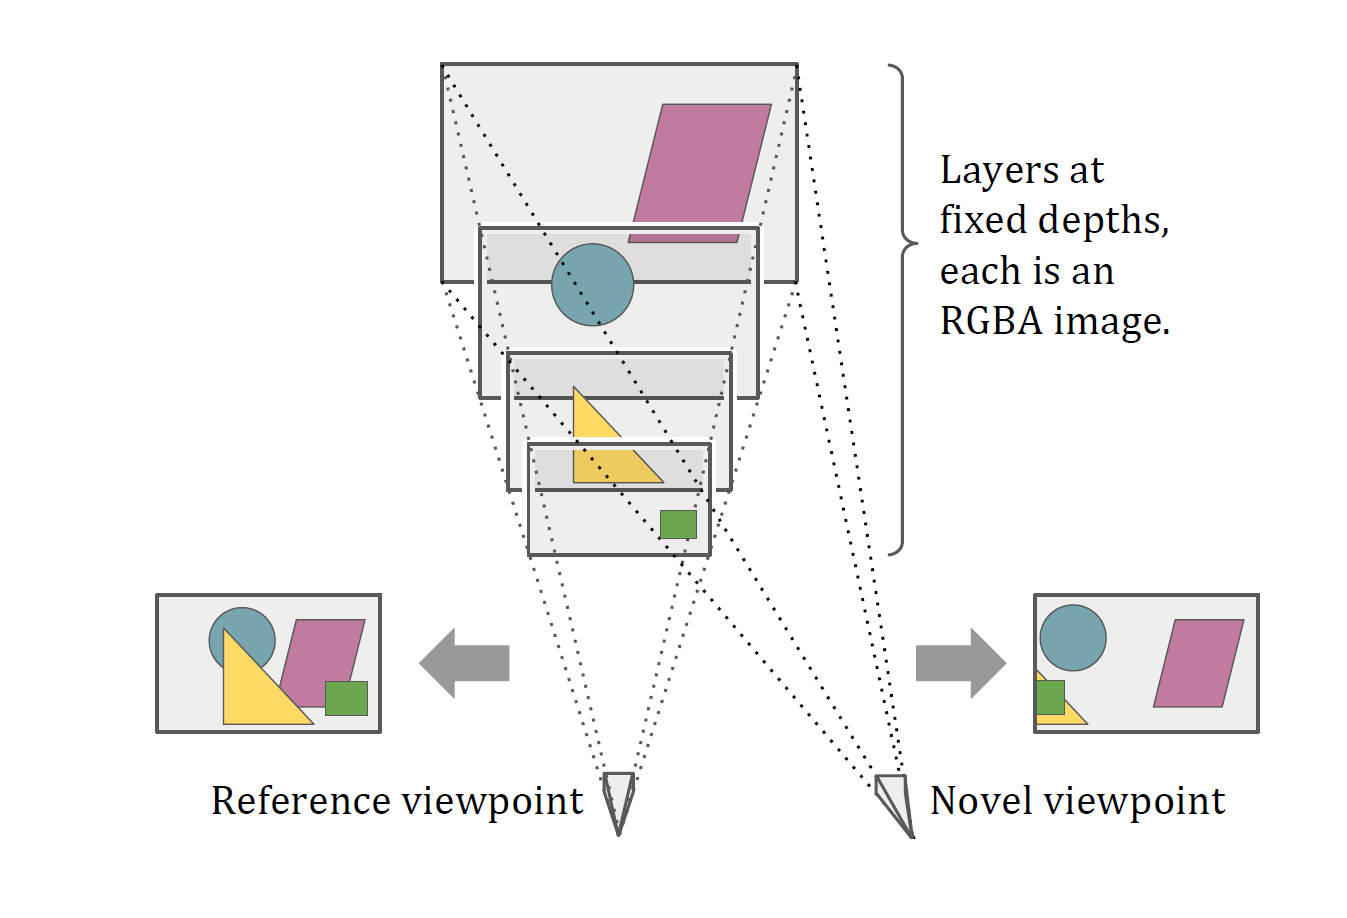
\includegraphics[width=1\columnwidth]{figures/mpi-layered-representation.png}
    \caption{Fronto-parallel planes in MPI layered representation}
    \label{fig:mpi-layered-representation}
\end{figure}
Fig 3. Example of fronto-parallel planes

However, in fact, the coordinates of picture dots cannot be determined with arbitrarily high precision. Rather than that, other sources of noise, such as geometric noise caused by lens distortion or interest point recognition mistake, cause inconsistencies in the picture coordinates that are measured. As a result, the lines created by the associated picture points do not always meet in three-dimensional space. The objective is then to identify a three-dimensional point that fits the observed picture points optimally. Numerous approaches exist in the literature for how to define optimality and how to determine the optimal 3D location. Due to the fact that the various approaches are based on distinct optimality criteria, they generate significantly varied estimations of the 3D point x when noise is present.

tringulation slides on onedrive for diagram
https://en.wikipedia.org/wiki/Triangulation_(computer_vision)
https://www.sciencedirect.com/topics/engineering/disparity-map
https://en.wikipedia.org/wiki/Binocular_disparity
single view or monocular